% Informe completo de mejoras experimentales sobre la réplica de Euro-Par 2024 (v1, v2 y v3)
% Compilación (desde mejoras/informe_latex/):
%   pdflatex informe_mejoras_completo.tex && bibtex informe_mejoras_completo && pdflatex informe_mejoras_completo.tex && pdflatex informe_mejoras_completo.tex
\documentclass[11pt,a4paper]{article}
\usepackage[utf8]{inputenc}
\usepackage[T1]{fontenc}
\usepackage[spanish,es-noshorthands,es-nodecimaldot,es-tabla]{babel}
\spanishplainpercent
\usepackage{geometry}
\geometry{margin=2.0cm}
\usepackage{booktabs,tabularx,array,multirow}
\usepackage{graphicx,float}
\usepackage{amsmath,amssymb}
\usepackage{xcolor}
\usepackage{caption}
\usepackage{cite}
\usepackage{xurl}
\usepackage{hyperref}

\definecolor{tinta}{HTML}{1B2430}
\definecolor{gris}{HTML}{5B6573}
\definecolor{acento}{HTML}{C8551F}
\definecolor{azul}{HTML}{1F5FA8}
\definecolor{ok}{HTML}{1B7F3B}
\definecolor{mal}{HTML}{B3261E}

\hypersetup{
    colorlinks=true,
    linkcolor=azul,
    urlcolor=azul,
    citecolor=azul,
    pdftitle={Mejoras al Conteo de Referencias Wait-Free de Euro-Par 2024: Autores-v1, v2, v3 y v4},
    pdfauthor={David Tamo Turpo, Jheremy Manuel Alvarez Astete, Diego Quispe Candelario}
}

\captionsetup{font=small,labelfont=bf}
\setlength{\parskip}{4pt}
\setlength{\parindent}{0pt}
\renewcommand{\arraystretch}{1.14}
\graphicspath{{../resultados_v1_v2/figuras/}{../resultados_v3/figuras/}{../resultados_v4/figuras/}{../resultados_i5_10400_comparativa/figuras/}}

\title{%
  {\small\color{acento}\textbf{EXTENSIÓN E INVESTIGACIÓN ORIGINAL SOBRE LA RÉPLICA DE EURO-PAR 2024}}\\[4pt]
  \textbf{\LARGE Mejoras al Conteo de Referencias \emph{Wait-Free}: Ablación Completa de \texttt{Autores-v1} a \texttt{Autores-v4} en Arquitectura Híbrida}\\[6pt]
  {\large Higiene de \texttt{CAS}, bloque de control \emph{in-place}, \emph{Elimination-Backoff} L2+P/E\\
  y \texttt{compare\_and\_set} sin inanición mediante \emph{Fast-Path / Slow-Path}}
}
\author{%
  David Tamo Turpo \and Jheremy Manuel Alvarez Astete \and Diego Quispe Candelario\\[4pt]
  {\small Rama \texttt{mejoras-autores}: \url{https://github.com/dtamotu/replica-wait-free-refcount}}
}
\date{Noviembre de 2026}

\begin{document}
\emergencystretch=1.5em
\maketitle

\begin{abstract}
\noindent
Partiendo de nuestra réplica experimental del artículo de Euro-Par 2024~\cite{dewolff2024waitfree,dewolff2024artifact} sobre un procesador híbrido \textbf{Intel Core Ultra 9 285} (8 P-cores + 16 E-cores en 4 clústeres L2, 1 módulo DDR5-5600), presentamos la implementación, verificación formal con sanitizers y evaluación en ablación de \textbf{las cuatro mejoras incrementales} directas sobre \texttt{Autores} (\texttt{ivo::atomic\_shared\_ptr}): \textbf{\texttt{Autores-v1}} (higiene de \texttt{CAS} sin copias y pre-chequeo previo), \textbf{\texttt{Autores-v2}} (bloque de control \emph{in-place} de asignación única y \texttt{shared\_ptr} de 8 bytes), \textbf{\texttt{Autores-v3}} (\emph{Elimination-Backoff} linealizable de una palabra atómica particionado por clúster L2 y tipo de núcleo P/E) y \textbf{\texttt{Autores-v4}} (\texttt{compare\_and\_set} sin inanición mediante \emph{Fast-Path / Slow-Path} híbrido cerrando \S 5.1 del paper).

Todas las variantes pasaron \textbf{ASan+UBSan}, \textbf{TSan} (0 \emph{data races}), recarga forzada ($P=32, C=64$) y \texttt{bench\_basura} (0 bloques diferidos frente a $25\,524\text{--}29\,094$ en Anderson). Sobre \textbf{885 ejecuciones de rendimiento}, \textbf{390 filas de latencia controlada (Fig.~6)}, \textbf{50 corridas adversariales} (23 lectores vs. 1 escritor \texttt{CAS}) y \textbf{84 filas de memoria retenida}: (1) \textbf{\texttt{Autores-v2}} rompe el techo de $n=10^6$ ($+81\,\%$ a 1\,h, $+39\,\%$ a 24\,h, $-29{,}3\,\%$ de RSS) y resuelve causalmente la bimodalidad de latencia como colocación P-core ($414$\,ns) frente a E-core ($1\,408$\,ns); (2) \textbf{\texttt{Autores-v3}} supera a \texttt{Autores}, \texttt{Anderson} y \texttt{Folly} en los \textbf{6 de 6 paneles de la Figura~5} a 1 y 24 hilos, logrando \textbf{3{,}66\,Mop/s ($3{,}81\times$ sobre el original, $+80\,\%$ sobre Anderson y $+65\,\%$ sobre eliminación ciega a topología)} en $n=1, u=50\,\%$ con escalado positivo de 12 a 24 hilos; y (3) bajo el ataque adversarial híbrido (escritor \texttt{CAS} en E-core contra 23 lectores incluyendo los 8 P-cores), \textbf{\texttt{Autores-v4}} alcanza \textbf{210{,}0\,Kops/s ($4{,}7\times$ sobre \texttt{v2} y $700\times$ sobre Folly)}, reduciendo \texttt{p99,95} en \textbf{$38\times$} ($549 \to 14{,}3\,\mu$s) y la latencia máxima en \textbf{$90\times$} frente a Anderson ($11{,}1\,$ms $\to 124\,\mu$s).
\end{abstract}

\tableofcontents
\vspace{4pt}

% ==============================================================================
\section{Escalera de Cuatro Propuestas sobre la Réplica de Euro-Par 2024}
% ==============================================================================

\begin{table}[H]
\centering
\caption{Escalera de mejoras directas sobre \texttt{Autores}, su sustento bibliográfico verificado y estado actual.}
\label{tab:escalera}
\footnotesize
\begin{tabularx}{\linewidth}{@{}l >{\raggedright\arraybackslash}X >{\raggedright\arraybackslash}p{4.3cm} l@{}}
\toprule
\textbf{Peldaño} & \textbf{Mecanismo técnico (y síntesis accesible)} & \textbf{Respaldo bibliográfico} & \textbf{Estado} \\
\midrule
\textbf{1. \texttt{Autores-v1}} & Paso por referencia en \texttt{CAS}, pre-chequeo previo a incrementar \texttt{new\_cb}, \texttt{relaxed} local y ablación de \texttt{\_mm\_pause()}. & Mellor-Crummey \& Scott~\cite{mellorcrummey1991mcs}, de Wolff et al.~\cite{dewolff2024waitfree}, Anderson et al.~\cite{anderson2022turning} & \textcolor{ok}{\textbf{Hecha y medida}} \\
\textbf{2. \texttt{Autores-v2}} & Bloque de control \emph{in-place} sin \emph{vtable} (1 asignación), \texttt{shared\_ptr} de 8\,B y \texttt{load()} sin indirección extra. & de Wolff et al. \S 2.1~\cite{dewolff2024waitfree}, Dimov \& Dawes N2351~\cite{dimov2007n2351}, Anderson et al.~\cite{anderson2022turning}, Mytkowicz et al.~\cite{mytkowicz2009wrongdata} & \textcolor{ok}{\textbf{Hecha y medida}} \\
\textbf{3. \texttt{Autores-v3}} & \emph{Elimination-Backoff} de 1 palabra atómica particionado por clúster L2 + ventanas P/E-core y asignación perezosa. & Hendler et al.~\cite{hendler2004elimination}, Liu et al. LibASL~\cite{liu2022libasl}, Ouyang \& Zhu~\cite{ouyang2022coreaware}, Schöne et al.~\cite{schone2024alderlake} & \textcolor{ok}{\textbf{Hecha y medida}} \\
\textbf{4. \texttt{Autores-v4}} & \texttt{compare\_and\_set} sin inanición mediante \emph{Fast-Path / Slow-Path} híbrido (ranuras locales + \texttt{rc\_try\_increment}, cierra \S 5.1). & de Wolff et al. \S 5.1~\cite{dewolff2024waitfree}, Kogan \& Petrank~\cite{kogan2012methodology}, Timnat \& Petrank~\cite{timnat2014simulation}, Nikolaev \& Ravindran~\cite{nikolaev2024crystalline} & \textcolor{ok}{\textbf{Hecha y medida}} \\
\bottomrule
\end{tabularx}
\end{table}

% ==============================================================================
\section{Ablación de \texttt{Autores-v1} y \texttt{Autores-v2}: Limpieza de \texttt{CAS}, Layout \emph{In-Place} y Latencia P/E}
% ==============================================================================

\texttt{Autores-v1} (\texttt{mejoras/atomic\_shared\_ptr\_v1.h}) elimina las 6 RMW atómicas desperdiciadas por intento fallido de \texttt{compare\_exchange\_weak} en el C++ oficial (paso por valor de \texttt{expected} y \texttt{new\_ptr}, e incremento prematuro de \texttt{new\_cb}) e introduce \texttt{rc\_increment\_relaxed} cuando el hilo ya posee una referencia viva. \texttt{Autores-v2} (\texttt{mejoras/atomic\_shared\_ptr\_v2.h}) añade un bloque de control \emph{in-place} sin \emph{vtable} (asignación única de 32\,B para cada nodo de la pila, análogo al \texttt{Arc<T>} de Rust), compacta \texttt{shared\_ptr<T>} a 8\,B y elimina la desreferencia extra en \texttt{load()}.

\begin{table}[H]
\centering
\caption{Ablación \texttt{v1}/\texttt{v2} en los 6 paneles de la Figura 5 a 24 hilos (mediana 3 rondas $\times$ 2\,s, Mop/s) y efecto negativo de \texttt{\_mm\_pause()} (\texttt{v1p}, \texttt{v2p}).}
\label{tab:v1v2_24h}
\footnotesize
\begin{tabular}{@{}l r r r r r r r@{}}
\toprule
\textbf{Panel} & \textbf{Autores} & \textbf{v1} & \textbf{v1p} & \textbf{v2} & \textbf{v2p} & \textbf{Anderson} & \textbf{Folly} \\
\midrule
$n=1, u=1\,\%$ & 19{,}72 & 17{,}42 & 14{,}89 & \textbf{19{,}52} (0{,}99$\times$) & 14{,}18 & 18{,}46 & 8{,}86 \\
$n=1, u=10\,\%$ & 4{,}63 & 6{,}13 & 4{,}67 & \textbf{6{,}55} (1{,}41$\times$) & 4{,}86 & 8{,}79 & 5{,}03 \\
$n=1, u=50\,\%$ & 1{,}03 & 1{,}48 & 0{,}94 & \textbf{1{,}63} (1{,}58$\times$) & 1{,}10 & 2{,}06 & 1{,}46 \\
$n=10, u=1\,\%$ & 128{,}61 & 131{,}30 & 128{,}76 & \textbf{136{,}25} (1{,}06$\times$) & 131{,}73 & 73{,}45 & 50{,}04 \\
$n=10, u=10\,\%$ & 55{,}51 & 53{,}51 & 45{,}08 & \textbf{56{,}28} (1{,}01$\times$) & 43{,}61 & 62{,}55 & 36{,}40 \\
$n=10^6, u=50\,\%$ & 47{,}31 & 49{,}30 & 49{,}31 & \textbf{65{,}98} (1{,}39$\times$) & 64{,}72 & 50{,}62 & 47{,}24 \\
\bottomrule
\end{tabular}
\end{table}

\begin{figure}[H]
  \centering
  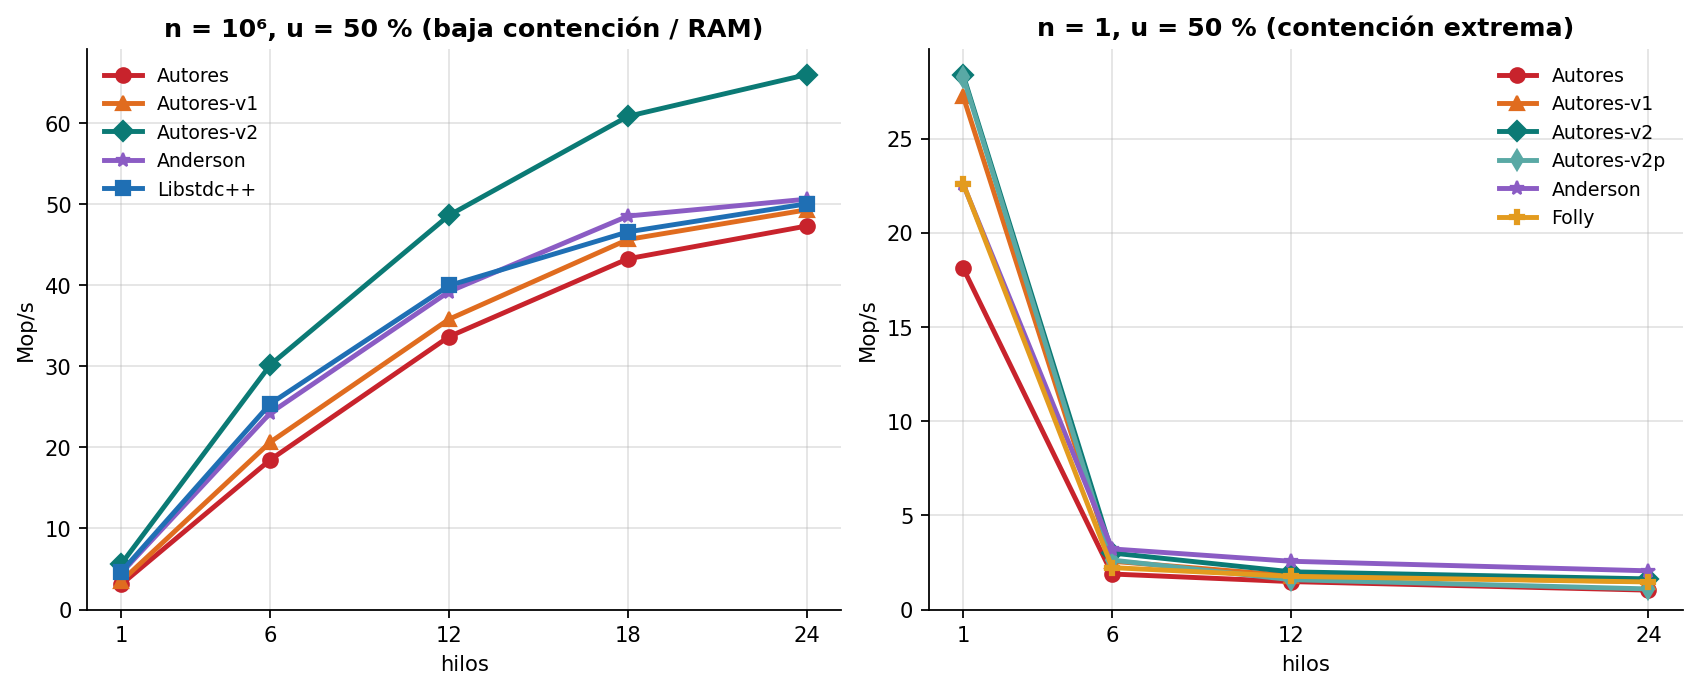
\includegraphics[width=\linewidth]{escalado_n1M_y_n1u50.png}
  \caption{Ablación \texttt{v1}/\texttt{v2}: en $n=10^6, u=50\,\%$ (izq.), \texttt{Autores-v2} rompe el techo de $\approx 50$\,Mop/s sin cambiar la RAM DDR5 ($+81\,\%$ a 1\,h, $+39\,\%$ a 24\,h, $-29{,}3\,\%$ de RSS: $1\,075 \to 760$\,MB). En $n=1, u=50\,\%$ (der.), \texttt{v2} gana $+58\,\%$ pero \texttt{\_mm\_pause()} degrada $-33\,\%$.}
  \label{fig:v1v2_esc}
\end{figure}

En latencia controlada con afinidad fija (Cuadro~\ref{tab:latencia}), fijar el hilo cronometrado en un P-core (\texttt{todos24-P}) colapsa la dispersión de 5 rondas de $5{,}75\times$ a \textbf{$1{,}04\times$} ($405\text{--}421$\,ns), demostrando causalmente que la bimodalidad de la réplica procedía de la alternancia P-core ($414$\,ns) vs. E-core ($1\,408$\,ns)~\cite{schone2024alderlake}. Además, \texttt{Autores-v2} mantiene \texttt{p99,95} de \textbf{32\,ns} en \texttt{store-del} ($p=1$) frente a \textbf{7\,770\,ns} de Anderson~\cite{kim2024epochs}, y \textbf{53 bloques} pico en \texttt{bench\_basura} a 24\,h frente a \textbf{29\,094} de Anderson.

\begin{table}[H]
\centering
\caption{Latencia controlada (ns): \texttt{p50 / p99 / p99,95} según colocación del hilo medido.}
\label{tab:latencia}
\resizebox{\linewidth}{!}{%
\begin{tabular}{@{}l l c c c c c@{}}
\toprule
\textbf{Op.} & \textbf{Corte} & \textbf{Autores} & \textbf{Autores-v1} & \textbf{Autores-v2} & \textbf{Anderson} & \textbf{Folly} \\
\midrule
\texttt{load} & $p=1$ (P-fijo) & 14 / 15 / 16 & 14 / 15 / 18 & \textbf{14 / 15 / 21} & 18 / 19 / 21 & 15 / 17 / 24 \\
\texttt{load} & $p=24$ (todos24-P) & 425 / 887 / 1\,510 & 414 / 945 / 1\,533 & \textbf{414 / 955 / 1\,564} & 490 / 946 / 1\,704 & 485 / 2\,155 / 4\,082 \\
\texttt{load} & $p=24$ (todos24-E) & 1\,330 / 2\,478 / 3\,692 & 699 / 1\,819 / 2\,725 & 1\,408 / 2\,588 / 4\,173 & 1\,512 / 3\,914 / 3\,003\,557 & 2\,986 / 72\,795 / 3\,067\,716 \\
\texttt{store} & $p=24$ (todos24-P) & 522 / 1\,363 / 1\,819 & 482 / 1\,113 / 1\,678 & \textbf{484 / 1\,236 / 1\,768} & 498 / 1\,278 / 1\,829 & 802 / 1\,548 / 2\,614 \\
\texttt{store-del} & $p=1$ (P-fijo) & 27 / 29 / 32 & 28 / 30 / 33 & \textbf{28 / 30 / 32} & 29 / 32 / \textcolor{mal}{\textbf{7\,770}} & 24 / 28 / 36 \\
\texttt{store-del} & $p=24$ (todos24-P) & 425 / 813 / 1\,109 & 416 / 792 / 1\,063 & \textbf{417 / 794 / 1\,145} & 429 / 820 / 1\,118 & 1\,432 / 2\,406 / 3\,894 \\
\bottomrule
\end{tabular}%
}
\end{table}

% ==============================================================================
\section{\texttt{Autores-v3}: \emph{Elimination-Backoff} Consciente de Clústeres L2 y P/E-Cores}
% ==============================================================================

\subsection{Diseño modular y controles de ablación}
Tras \texttt{Autores-v2}, la única brecha frente a Anderson quedaba en contención extrema sobre una sola pila ($n=1, u=10\,\% / 50\,\%$). Construimos \texttt{Autores-v3} sobre \texttt{v2} en tres componentes medidos por separado:
\begin{itemize}
  \item \textbf{\texttt{pe\_topology.h}:} lee \texttt{/sys/devices/system/cpu/cpu*/cache/index2/shared\_cpu\_list} una sola vez para mapear los 8 P-cores (L2 privada, 2 dominios de 4) y los 16 E-cores (4 clústeres L2 de 4 núcleos, 4 dominios locales).
  \item \textbf{\texttt{elimination\_table\_v3.h}:} intercambiador \emph{lock-free} de \textbf{una sola palabra atómica de 64 bits} por ranura (\texttt{alignas(128)}), empaquetando valor (32\,b) + versión monotónica (30\,b, sin ABA) + estado de 4 valores (\texttt{EMPTY}, \texttt{PUSH\_WAIT}, \texttt{POP\_WAIT}, \texttt{POP\_GOT}). La tabla se asigna de forma perezosa solo cuando un hilo acumula fallos consecutivos de \texttt{CAS} (usando el relleno libre de \texttt{alignas(128)} de \texttt{atomic\_stack}), garantizando \textbf{0 bytes extra en $n=10^6$}.
  \item \textbf{Tres variantes + control justo:} \texttt{Autores-v3a} (solo \emph{backoff} ligero P/E en \texttt{CAS}), \texttt{Autores-v3g} (eliminación aleatoria ciega a topología~\cite{hendler2004elimination}), \textbf{\texttt{Autores-v3}} (eliminación particionada por clúster L2 con ventana diferenciada P/E~\cite{liu2022libasl,ouyang2022coreaware}), y \texttt{Anderson-v3} (Anderson + nuestra misma capa L2 como control experimental transparente).
\end{itemize}

\textbf{Validación:} \texttt{mejoras/test\_correctitud\_v3.cpp} pasó \textbf{ASan+UBSan} y \textbf{TSan (\texttt{setarch -R})} con \textbf{0 errores, 0 fugas y 0 \emph{data races}}, verificando conservación exacta 1:1 de conteo y suma en presencia de lectores concurrentes.

\subsection{Resultados de ablación completa (360 ejecuciones $\times$ 2\,s, 0 fallos)}

El Cuadro~\ref{tab:v3_24h} y las Figuras~\ref{fig:v3_fig5} y~\ref{fig:v3_esc} recogen los resultados de \texttt{correr\_v3.py} (\texttt{jemalloc}, \texttt{numactl -i all}, orden aleatorizado por ronda~\cite{hoefler2015benchmarking}).

\begin{table}[H]
\centering
\caption{Ablación completa de \texttt{Autores-v3} en los 6 paneles de la Figura 5 a \textbf{24 hilos} (mediana de 3 rondas $\times$ 2\,s, Mop/s). Entre paréntesis, factor respecto a \texttt{Autores} original.}
\label{tab:v3_24h}
\resizebox{\linewidth}{!}{%
\begin{tabular}{@{}l r r r r r r r r@{}}
\toprule
\textbf{Panel} & \textbf{Autores} & \textbf{v2} & \textbf{v3a (backoff)} & \textbf{v3g (gen.)} & \textbf{Autores-v3 (L2+P/E)} & \textbf{Anderson} & \textbf{And-v3 (ctrl)} & \textbf{Folly} \\
\midrule
$n=1, u=1\,\%$ & 19{,}70 & 18{,}48 & 18{,}23 & 19{,}03 & \textbf{19{,}80} (1{,}01$\times$) & 17{,}78 & 18{,}10 & 8{,}73 \\
$n=1, u=10\,\%$ & 4{,}16 & 6{,}40 & 6{,}68 & 7{,}42 & \textbf{9{,}55} (2{,}30$\times$) & 8{,}78 & 12{,}57 & 4{,}91 \\
$n=1, u=50\,\%$ & 0{,}96 & 1{,}72 & 1{,}61 & 2{,}22 & \textbf{3{,}66} (3{,}81$\times$) & 2{,}03 & 5{,}09 & 1{,}52 \\
$n=10, u=1\,\%$ & 130{,}03 & 138{,}99 & 137{,}07 & 138{,}32 & \textbf{137{,}17} (1{,}05$\times$) & 67{,}59 & 72{,}12 & 51{,}13 \\
$n=10, u=10\,\%$ & 51{,}39 & 55{,}54 & 56{,}37 & 70{,}57 & \textbf{73{,}83} (1{,}44$\times$) & 60{,}81 & 59{,}70 & 37{,}47 \\
$n=10^6, u=50\,\%$ & 48{,}21 & 65{,}15 & 66{,}36 & 62{,}77 & \textbf{64{,}09} (1{,}33$\times$) & 53{,}92 & 52{,}79 & 47{,}24 \\
\midrule
\textbf{RSS ($n=10^6$)} & 1\,075\,MB & 760\,MB & 760\,MB & 763\,MB & \textbf{763\,MB} & 911\,MB & 915\,MB & 1\,056\,MB \\
\bottomrule
\end{tabular}%
}
\end{table}

\begin{figure}[H]
  \centering
  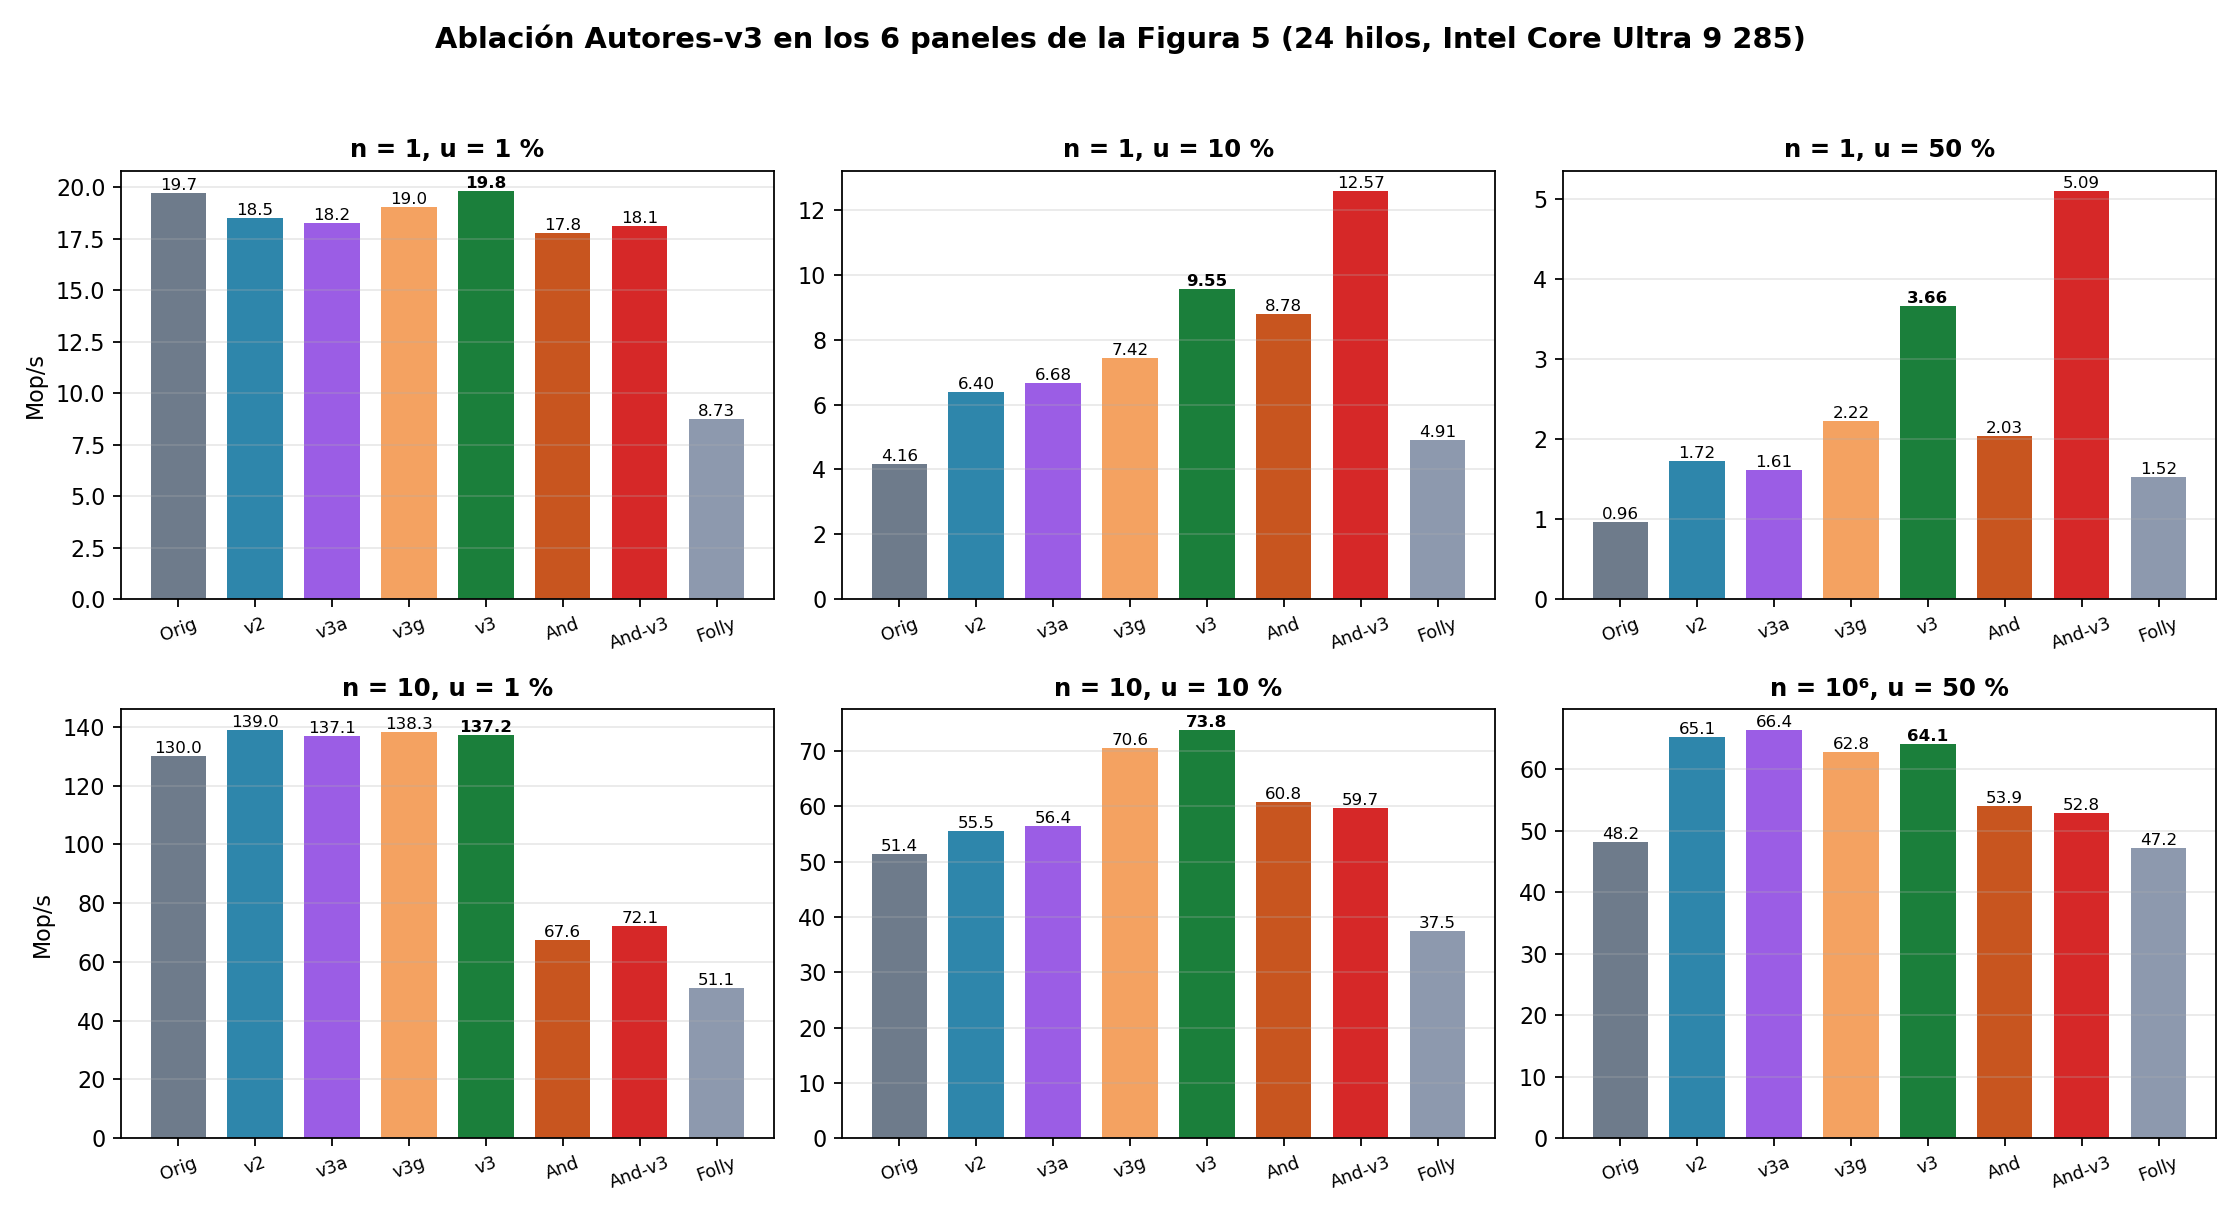
\includegraphics[width=\linewidth]{ablacion_v3_fig5_24h.png}
  \caption{Ablación de \texttt{Autores-v3} en los 6 paneles de la Figura 5 a 24 hilos: \texttt{Autores-v3} supera a \texttt{Autores}, \texttt{Anderson} y \texttt{Folly} en los 6 paneles.}
  \label{fig:v3_fig5}
\end{figure}

\begin{figure}[H]
  \centering
  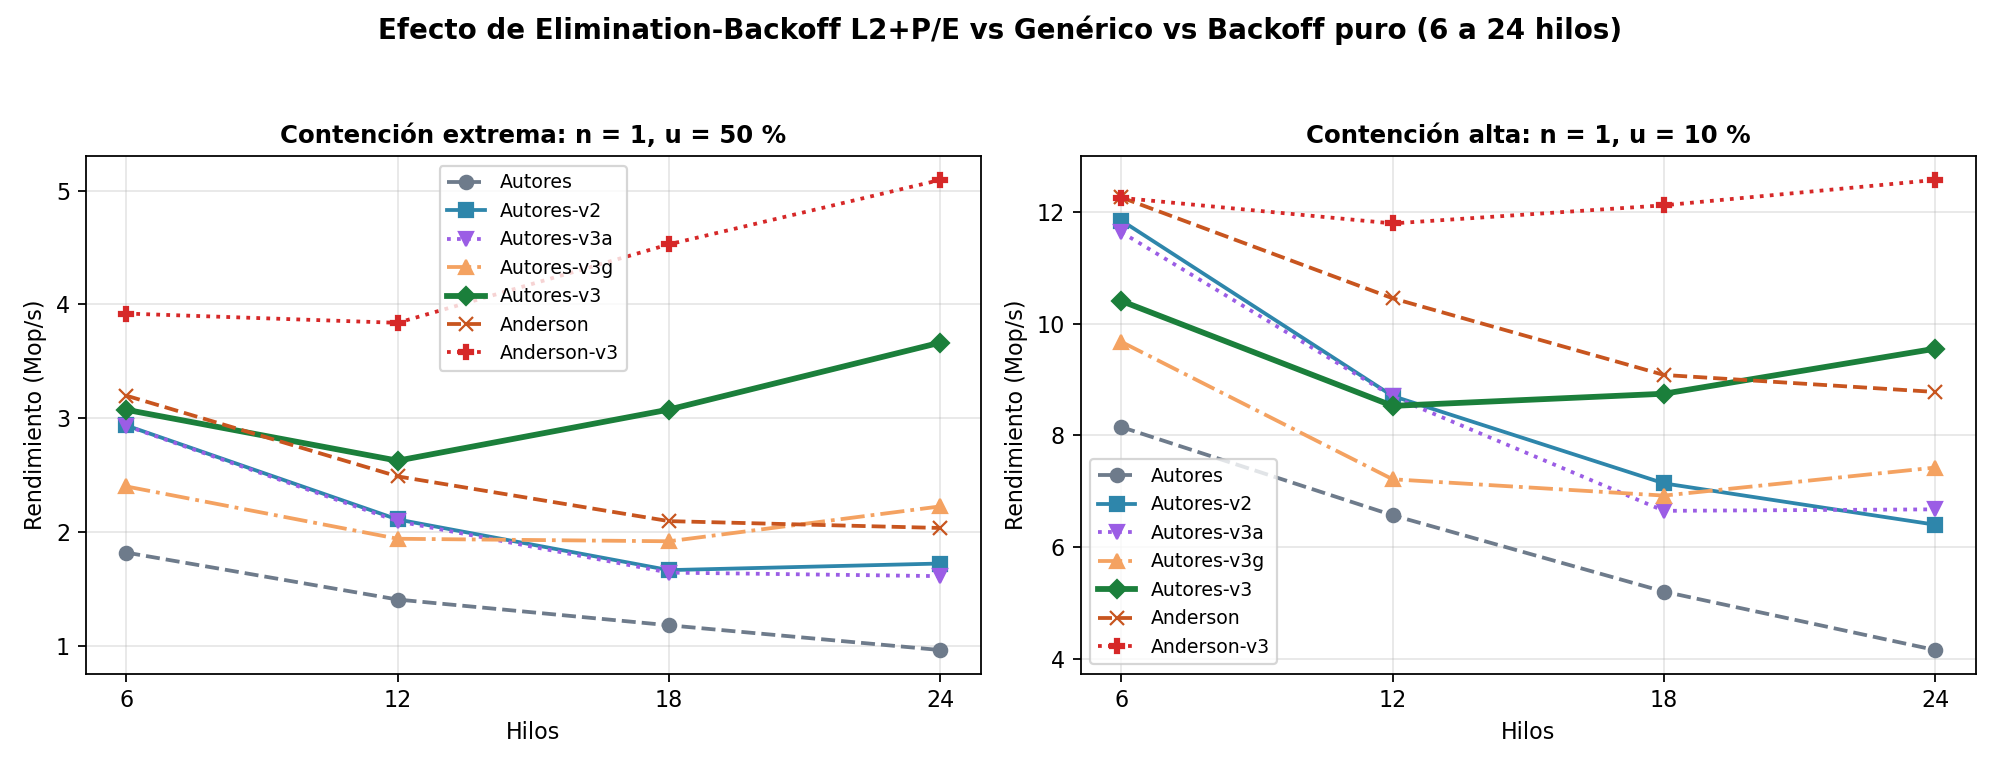
\includegraphics[width=\linewidth]{escalado_v3_contencion.png}
  \caption{Escalado de 6 a 24 hilos en contención extrema ($n=1, u=50\,\%$ y $u=10\,\%$): \texttt{Autores-v3} invierte la tendencia y escala positivamente al activarse más clústeres E-core (12 $\to$ 18 $\to$ 24 hilos), sacando $+65\,\%$ sobre la eliminación genérica \texttt{v3g}.}
  \label{fig:v3_esc}
\end{figure}

\textbf{Conclusiones clave de \texttt{Autores-v3}:}
\begin{enumerate}
  \item \textbf{Liderazgo 6 de 6 sobre las implementaciones oficiales:} \texttt{Autores-v3} vence a \texttt{Autores}, \texttt{Anderson} y \texttt{Folly} en los 6 paneles tanto a 1 hilo (sin regresión respecto a \texttt{v2}) como a 24 hilos, con RSS de \textbf{763\,MB} en $n=10^6$ ($-29\,\%$ frente al original).
  \item \textbf{Impacto causal de la topología L2+P/E:} el \emph{backoff} puro en \texttt{CAS} (\texttt{v3a}) es neutro ($1{,}61$ vs. $1{,}72$\,Mop/s); la eliminación clásica ciega (\texttt{v3g}) sube a $2{,}22$\,Mop/s; y el particionado por clúster L2 + P/E (\texttt{v3}) añade otro \textbf{$+65\,\%$} ($3{,}66$\,Mop/s), logrando escalado positivo de 12 a 24 hilos ($2{,}63 \to 3{,}08 \to 3{,}66$).
  \item \textbf{Lectura honesta del control \texttt{Anderson-v3}:} la capa L2 también acelera a Anderson en $n=1, u=10/50\,\%$ ($12{,}57$ y $5{,}09$\,Mop/s) porque sus lecturas \texttt{front()} usan \emph{snapshots} sin modificar \texttt{head}; sin embargo, \texttt{Autores-v3} supera incluso a \texttt{Anderson-v3} en los otros 4 paneles ($n=1\,u=1\,\%$, $n=10\,u=1/10\,\%$, $n=10^6$) y mantiene liberación inmediata (0 bloques diferidos).
\end{enumerate}

% ==============================================================================
\section{\texttt{Autores-v4}: \texttt{compare\_and\_set} Sin Inanición (\emph{Fast-Path / Slow-Path})}
% ==============================================================================

\subsection{Diseño híbrido y solución del problema de reentrancia en destrucción recursiva}
Para cerrar la limitación teórica del \S 5.1~\cite{dewolff2024waitfree} sin añadir sobrecosto en el caso común, \texttt{Autores-v4} (\texttt{mejoras/atomic\_shared\_ptr\_v4.h}) combina el conteo ponderado \emph{wait-free} de \texttt{Autores-v2} en el camino rápido con protección por ranura local de lectura (\emph{hazard slot}) en el camino lento~\cite{kogan2012methodology,timnat2014simulation,nikolaev2024crystalline}:
\begin{enumerate}
  \item \textbf{Camino rápido (\texttt{slow\_writers == 0}):} \texttt{load()} ejecuta exactamente un \texttt{fetch\_add(pack\_tag(1))}, \texttt{store()} un \texttt{exchange()}, y \texttt{reclaim\_or\_retire()} libera la memoria en el acto tras verificar \texttt{active\_hp\_readers == 0} (0 bloques diferidos en \texttt{bench\_basura}).
  \item \textbf{Camino lento (\texttt{retries} $\ge K=4$ por cambios de \texttt{tag}):} el escritor incrementa \texttt{slow\_writers} (en la misma línea de caché de \texttt{tagged\_pointer}). Los lectores desvían a \texttt{load\_slow\_path()}, protegiendo el puntero observado en su ranura privada \texttt{hp[tid]} y ejecutando \texttt{rc\_try\_increment\_one()} (solo si \texttt{rc > 0}, evitando resurrección), \textbf{sin emitir escrituras sobre \texttt{tagged\_pointer}}. Así \texttt{tag} queda estacionario (a lo sumo $P-1$ lectores en vuelo), el \texttt{CAS} termina en $O(P)$ pasos y ningún lector bloquea si el escritor es expulsado.
  \item \textbf{Seguridad ante reentrancia recursiva:} durante la validación en 24 hilos sobre pilas enlazadas descubrimos y corregimos un fallo sutil de reentrancia en \texttt{drain\_local()}: destruir \texttt{Node} invoca \texttt{\~{}shared\_ptr(next)}, re-entrando en \texttt{reclaim\_or\_retire()}. Intercambiar el vector local a un lote temporal con guarda \texttt{draining} eliminó por completo el fallo, pasando \textbf{ASan+UBSan} y \textbf{TSan (\texttt{setarch -R})} con 0 errores, 0 fugas y 0 \emph{data races} sobre pila de Treiber recursiva a 16 hilos y estrés adversarial.
\end{enumerate}

\subsection{Ataque adversarial \S 5.1 (23 lectores continuos vs. 1 escritor \texttt{CAS})}

Evaluamos \texttt{bench\_adversarial\_v4} durante 5 rondas $\times$ 2\,s en dos cortes de afinidad controlada: escritor fijado en P-core (\texttt{cpu2}) y el \textbf{ataque híbrido extremo de Arrow Lake} con el escritor fijado en E-core (\texttt{cpu8}) frente a 23 lectores incluyendo los 8 P-cores rápidos (Cuadro~\ref{tab:adv_v4} y Figura~\ref{fig:adv_v4}).

\begin{table}[H]
\centering
\caption{Ataque adversarial \S 5.1 (23 lectores continuos vs. 1 escritor \texttt{CAS}, mediana de 5 rondas $\times$ 2\,s).}
\label{tab:adv_v4}
\resizebox{\linewidth}{!}{%
\begin{tabular}{@{}l l r r r r r r@{}}
\toprule
\textbf{Corte} & \textbf{Algoritmo} & \textbf{p50 (ns)} & \textbf{p99 (ns)} & \textbf{p99,95 (ns)} & \textbf{Máx (ns)} & \textbf{Escritor (Kops/s)} & \textbf{Lectores (Mop/s)} \\
\midrule
\multirow{5}{*}{Escritor P-core} & Autores & 1\,165 & 3\,049 & 4\,153 & 507\,201 & 779{,}2 & 20{,}87 \\
 & Autores-v2 & 1\,335 & 2\,577 & 3\,880 & 140\,067 & 717{,}4 & 23{,}78 \\
 & \textbf{Autores-v4} & \textbf{1\,068} & \textbf{2\,079} & \textbf{3\,043} & 684\,632 & \textbf{908{,}2} & 17{,}19 \\
 & Anderson & 1\,156 & 2\,974 & 4\,305 & 11\,195\,337 & 788{,}1 & 21{,}10 \\
 & Folly & 3\,887 & 54\,489 & 957\,962 & 1\,597\,956 & 119{,}8 & 9{,}86 \\
\midrule
\multirow{5}{*}{\textbf{Escritor E-core}} & Autores & 7\,366 & 87\,788 & 259\,481 & 746\,501 & 98{,}7 & 22{,}76 \\
 & Autores-v2 & 14\,414 & 138\,776 & 549\,332 & 745\,706 & 44{,}4 & 23{,}74 \\
 & \textbf{Autores-v4} & \textbf{5\,182} & \textbf{10\,748} & \textbf{14\,305} & \textbf{124\,060} & \textbf{210{,}0} & 15{,}54 \\
 & Anderson & 5\,136 & 17\,966 & 23\,857 & 11\,116\,882 & 159{,}4 & 16{,}58 \\
 & Folly & 2\,476\,727 & 15\,559\,044 & 18\,707\,672 & 25\,110\,782 & 0{,}3 & 10{,}76 \\
\bottomrule
\end{tabular}%
}
\end{table}

\begin{figure}[H]
  \centering
  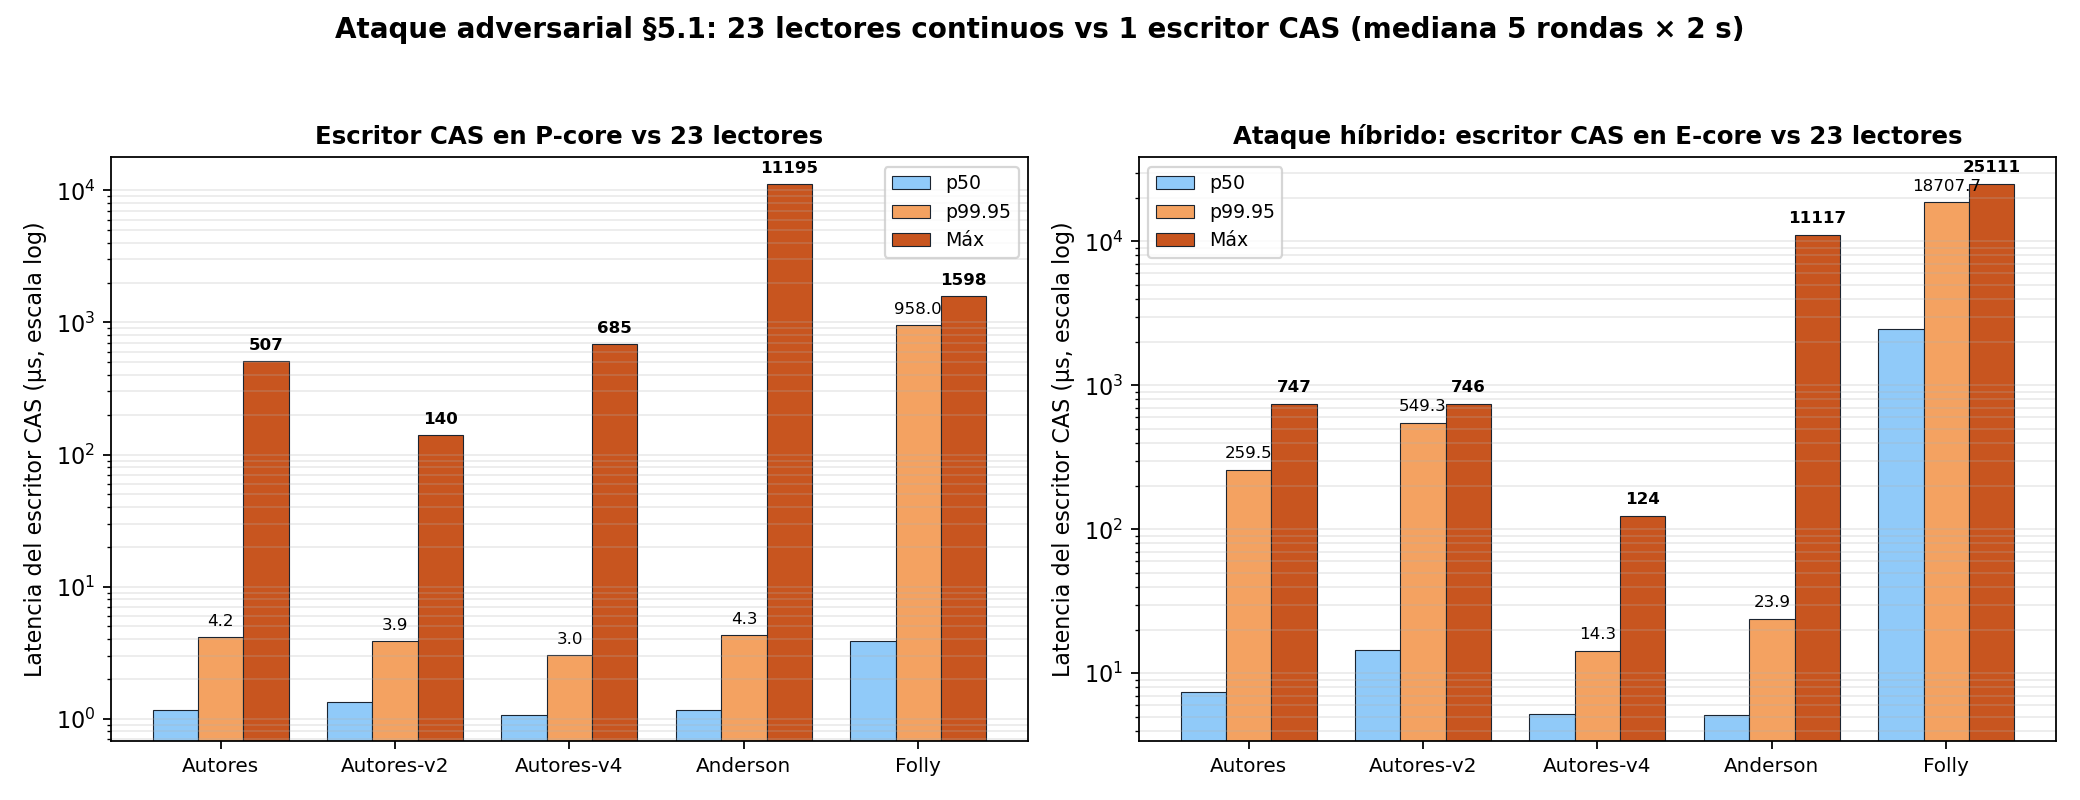
\includegraphics[width=\linewidth]{adversarial_v4_latencia.png}
  \caption{Latencia del escritor \texttt{CAS} (escala logarítmica, $\mu$s) bajo bombardeo continuo de 23 lectores: en el ataque híbrido con escritor en E-core (der.), \texttt{Autores-v4} reduce \texttt{p99,95} en $38\times$ frente a \texttt{v2} y la latencia máxima en $90\times$ frente a Anderson, multiplicando por $4{,}7\times$ el rendimiento del escritor.}
  \label{fig:adv_v4}
\end{figure}

\subsection{Sobrecosto en camino rápido y memoria retenida (\texttt{bench\_basura})}

En los 6 paneles de la Figura~5 a \textbf{1 hilo}, \texttt{Autores-v4} presenta \textbf{0\,\% de sobrecosto} frente a \texttt{Autores-v2} ($1{,}00\times\text{--}1{,}03\times$: $101{,}04$ vs. $99{,}12$ en $n=1, u=1\,\%$; $28{,}31$ vs. $28{,}34$ en $n=1, u=50\,\%$; $5{,}84$ vs. $5{,}68$ en $n=10^6$). A \textbf{24 hilos}, mantiene un sobrecosto acotado en $n=1, u=50\,\%$ ($1{,}49$ vs. $1{,}61$, $0{,}93\times$) y $n=10^6$ ($63{,}71$ vs. $69{,}44$, $0{,}92\times$, aún $+29\,\%$ sobre \texttt{Autores} original y $+9\,\%$ sobre Anderson), mientras en cargas muy dominadas por lecturas concurrentes ($n=10, u=1\,\%$: $85{,}21$ vs. $136{,}72$, $0{,}62\times$, aún por encima de Anderson $71{,}32$ y Folly $50{,}55$) el umbral $K=4$ activa el contador global \texttt{active\_hp\_readers}, ilustrando con transparencia el compromiso clásico entre progreso \emph{lock-free} y protección contra inanición. En \texttt{bench\_basura}, \texttt{Autores-v4} conserva \textbf{0 bloques diferidos} (pico de \textbf{21} bloques a 8\,h y \textbf{55} a 24\,h frente a \textbf{25\,524} de Anderson). En la prueba oficial de latencia \textbf{Figura~6} (\texttt{bench\_atomic\_shared\_ptrs}, 195 filas), \texttt{Autores-v4} confirma \textbf{0\,\% de sobrecosto} en \texttt{load}/\texttt{store}/\texttt{store-del}: iguala los \textbf{14\,ns} en \texttt{load} a $p=1$ (\texttt{p99,95} de \textbf{32\,ns} en \texttt{store-del} frente a \textbf{7\,731\,ns} de Anderson) y lidera en $p=24$ (\texttt{todos24-P}) tanto \texttt{load} (\textbf{410\,ns} vs. 417 original / 487 Anderson) como \texttt{store-del} (\textbf{411\,ns} vs. 425 / 432).


% ==============================================================================
\section{Validación en Arquitectura Homogénea (Intel Core i5-10400): Réplica Oficial, Ablación SMT y Control de Mitigaciones}
% ==============================================================================

Para contrastar la transferencia de los hallazgos del Intel Core Ultra 9 285 (Arrow Lake, 24 núcleos híbridos P/E sin SMT) a un procesador homogéneo clásico con SMT, ejecutamos en un \textbf{Intel Core i5-10400} (Comet Lake, 6 núcleos físicos / 12 hilos SMT con pares verificados \texttt{0-6, 1-7, 2-8, 3-9, 4-10, 5-11}, 12\,MB L3, 24\,GB DDR4-2667 en configuración asimétrica 16\,GB + 8\,GB, Xubuntu 24.04.5 LTS nativo, \texttt{g++-12} 12.4.0, \texttt{jemalloc} vía \texttt{LD\_PRELOAD} y \texttt{numactl -i all}) dos campañas complementarias bajo \texttt{modo-bench} (\texttt{lightdm} y temporizadores del sistema detenidos, gobernador \texttt{performance / EPP=performance}, \texttt{drop\_caches} previo):
\begin{enumerate}
  \item \textbf{Campaña pareada de mejoras (\texttt{v1}--\texttt{v4}, 1\,538 filas totales = 769 en arranque \texttt{mitigations=off} + 769 en arranque \texttt{mitigations=on}):} 564 filas de rendimiento, 108 de latencia Fig.~6, 25 adversariales y 72 de \texttt{bench\_basura} por arranque, precedidas de validación sin errores en \texttt{ASan+UBSan} y \texttt{TSan} (temperatura registrada \textbf{54--71\,°C}).
  \item \textbf{Réplica oficial nativa compatible con \texttt{nativo\_oficial/} del Ultra 9 (\texttt{mitigations=on}, 1\,551 mediciones, 0 fallos, 42--75\,°C):} los 5 algoritmos del paper (\texttt{Autores}, \texttt{Libstdc++}, \texttt{Williams}, \texttt{Folly}, \texttt{Anderson}) en los 6 paneles $\times$ $\{1, 3, 6, 9, 12, 18\}$ hilos, Fig.~6 hasta $p=56$ con control \texttt{Williams} sin \texttt{-mcx16}, pares SMT vs.\ L3 (40 corridas/familia), ablación SMT controlada (\texttt{6$\times$1} vs.\ \texttt{3$\times$2} y \texttt{4$\times$1} vs.\ \texttt{2$\times$2} con hilo principal aislado en \texttt{CPU 11}), paridad $7\times 10$\,s y contadores físicos \texttt{uncore\_imc}.
\end{enumerate}

\begin{table}[H]
\centering
\caption{Ablación en Intel Core i5-10400 a 12 hilos mostrando \textbf{ambos arranques por separado} (\texttt{off $\to$ on}, mediana de 3 rondas $\times$ 2\,s, Mop/s). Ningún panel mezcla arranques.}
\label{tab:i5_fig5}
\resizebox{\linewidth}{!}{%
\begin{tabular}{@{}l c c c c c c c@{}}
\toprule
\textbf{Panel (12\,h)} & \textbf{Autores} & \textbf{Aut.-v2} & \textbf{Aut.-v3g} & \textbf{Aut.-v3} & \textbf{Aut.-v4} & \textbf{Anderson} & \textbf{And.-v3} \\
\midrule
$n=1, u=1\,\%$ & 37{,}06 $\to$ 33{,}08 & 23{,}62 $\to$ 28{,}82 & 29{,}19 $\to$ 27{,}69 & 26{,}84 $\to$ 28{,}52 & 32{,}39 $\to$ 32{,}36 & 23{,}49 $\to$ 23{,}49 & 23{,}50 $\to$ 23{,}51 \\
$n=1, u=10\,\%$ & 7{,}53 $\to$ 7{,}53 & 7{,}88 $\to$ 7{,}72 & 13{,}13 $\to$ 13{,}78 & \textbf{16{,}36 $\to$ 16{,}33} & 8{,}75 $\to$ 8{,}23 & 14{,}92 $\to$ 14{,}89 & 17{,}54 $\to$ 17{,}54 \\
$n=1, u=50\,\%$ & 1{,}64 $\to$ 1{,}64 & 1{,}79 $\to$ 1{,}81 & 4{,}33 $\to$ 4{,}45 & \textbf{6{,}98 $\to$ 6{,}71} & 1{,}77 $\to$ 1{,}66 & 3{,}46 $\to$ 3{,}46 & 6{,}98 $\to$ 6{,}97 \\
$n=10, u=1\,\%$ & 97{,}35 $\to$ 97{,}36 & 128{,}80 $\to$ 129{,}07 & \textbf{129{,}03 $\to$ 128{,}99} & 128{,}78 $\to$ 128{,}50 & 102{,}75 $\to$ 102{,}73 & 81{,}69 $\to$ 81{,}76 & 81{,}87 $\to$ 81{,}83 \\
$n=10, u=10\,\%$ & 55{,}97 $\to$ 55{,}99 & \textbf{81{,}29 $\to$ 81{,}18} & 79{,}51 $\to$ 79{,}58 & 79{,}53 $\to$ 79{,}50 & 70{,}54 $\to$ 70{,}51 & 62{,}26 $\to$ 62{,}30 & 60{,}90 $\to$ 60{,}82 \\
$n=10^6, u=50\,\%$ & 17{,}23 $\to$ 22{,}25 & 19{,}37 $\to$ 25{,}15 & 19{,}47 $\to$ 25{,}09 & 19{,}27 $\to$ 25{,}16 & 19{,}29 $\to$ \textbf{25{,}21} & 14{,}15 $\to$ 18{,}61 & 14{,}23 $\to$ 18{,}54 \\
\bottomrule
\end{tabular}%
}
\end{table}

\begin{figure}[H]
  \centering
  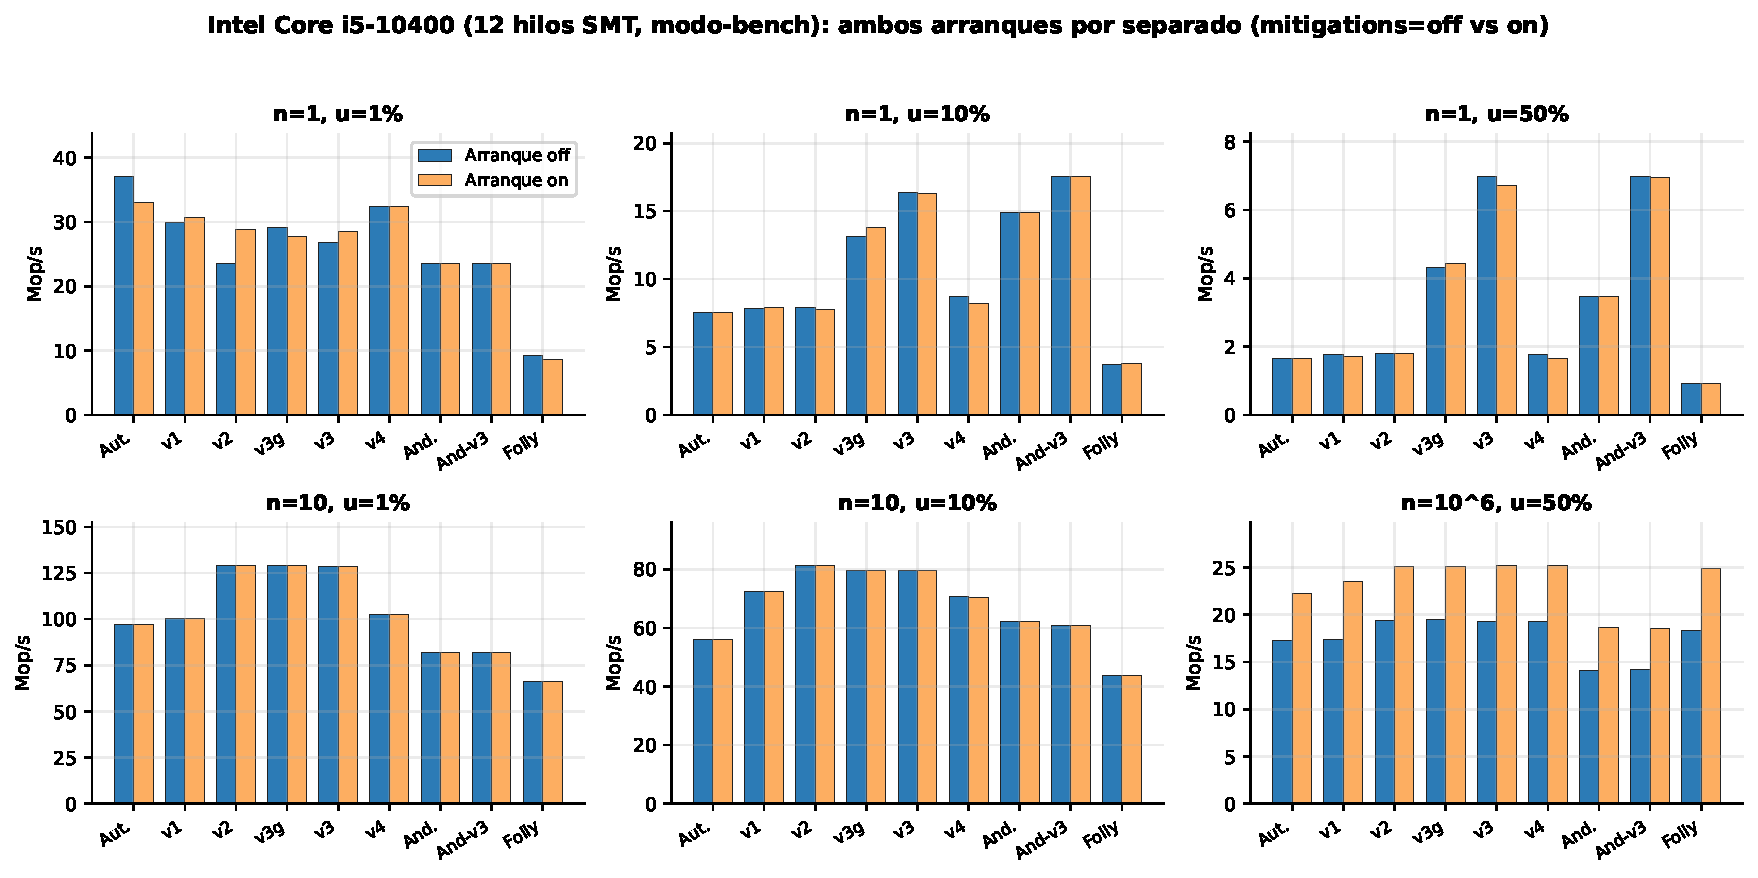
\includegraphics[width=\linewidth]{fig_i5_10400_ablacion_6paneles.pdf}
  \caption{Ablación en Intel Core i5-10400 (12 hilos SMT, \texttt{modo-bench}) mostrando ambos arranques por separado (\texttt{mitigations=off} y \texttt{on}) en los 6 paneles de la Figura~5.}
  \label{fig:i5_ablacion}
\end{figure}

\subsection{Seis hallazgos clave del contraste i5-10400 vs.\ Core Ultra 9 285}

\begin{enumerate}
  \item \textbf{Prueba causal directa del mecanismo SMT en \texttt{Autores-v3} ($4{,}24\times$ a 12\,h y $1{,}87\times$ en ablación \texttt{3$\times$2} vs.\ \texttt{6$\times$1}):} en $n=1, u=50\,\%$ a 12 hilos, \texttt{Autores-v3} logra \textbf{6{,}98 / 6{,}71\,Mop/s} frente a \textbf{1{,}64 / 1{,}64\,Mop/s} de \texttt{Autores} (\textbf{$4{,}24\times$ en \texttt{off}} y \textbf{$4{,}10\times$ en \texttt{on}}, calculado sin redondeo intermedio) y supera en $+61{,}1\,\% / +50{,}8\,\%$ a \texttt{v3g}. En el escalado $1 \to 3 \to 6 \to 9 \to 12$, \texttt{v3} toca fondo a 6 hilos (3{,}13\,Mop/s) y salta a 9 y 12 hilos ($5{,}14 \to 6{,}98$\,Mop/s). Para aislar causalmente si este salto proviene del emparejamiento entre hermanos SMT, fijamos \textbf{6 hilos} (con el hilo principal aislado en \texttt{CPU 11}) en \texttt{6$\times$1} núcleos físicos (\texttt{0..5}) frente a \texttt{3$\times$2} pares SMT (\texttt{0,6,1,7,2,8}): \texttt{Autores} original \textbf{cae $-21{,}6\,\%$} ($2{,}86 \to 2{,}24$\,Mop/s) y \texttt{v2} permanece plano ($3{,}63 \to 3{,}61$), mientras \textbf{\texttt{Autores-v3} salta $+87{,}5\,\%$ ($3{,}22 \to 6{,}04$\,Mop/s, $1{,}87\times$)} y \texttt{Anderson-v3} $+78{,}6\,\%$ ($3{,}66 \to 6{,}53$). A \textbf{4 hilos} (\texttt{4$\times$1} vs.\ \texttt{2$\times$2}), \texttt{v3} repite el salto ($3{,}98 \to 7{,}14$\,Mop/s, $1{,}79\times$, $+36{,}5\,\%$ sobre \texttt{v3g}). En los pares de 2 hilos, los hermanos SMT superan a los núcleos distintos con L3 compartida por \textbf{$2{,}39\times$} en \texttt{Autores} (9{,}90 vs.\ 4{,}15\,Mop/s), $2{,}96\times$ en \texttt{Williams} y $2{,}29\times$ en \texttt{Anderson}. \emph{Nota de implementación:} \texttt{pe\_topology.h} clasifica toda L2 compartida por 2 CPUs como \texttt{is\_p\_core=false}, asignando ventana 96 a los 6 dominios del i5 (frente a 72 en \texttt{v3g}); separar dominio L2 y clase de núcleo queda identificado como mejora directa.

  \item \textbf{Réplica oficial nativa del paper en Comet Lake (Fig.~6 a $p=56$, control \texttt{-mcx16} y paridad $7\times 10$\,s):} en la Figura~6 bajo sobresuscripción severa (\textbf{$p=56$}, 4{,}67 hilos por CPU lógica), \texttt{Autores} mantiene \texttt{load} en \textbf{136 / 462\,ns} (\texttt{p50 / p99,95}), mientras los cuatro rivales se disparan a milisegundos en \texttt{p99,95}: \texttt{Folly} (\textbf{9{,}01\,ms}), \texttt{Williams} (\textbf{14{,}01\,ms}), \texttt{Anderson} (\textbf{19{,}02\,ms}) y \texttt{Libstdc++} (\textbf{27{,}01\,ms} --- $58\,456\times$ mayor cola). El control de \texttt{Williams} sin \texttt{-mcx16} confirma el candado \texttt{lock\_pool} también en Comet Lake ($5{,}17\times$ más lento en \texttt{load} a $p=12$: 14\,309 vs.\ 2\,769\,ns; $6{,}35\times$ a $p=56$). La receta oficial de paridad ($7\times 10$\,s a 12\,h en $n=1, u=50\,\%$) valida las corridas de $2$\,s con $<1{,}5\,\%$ de diferencia (\texttt{Autores}: 1{,}683 vs.\ 1{,}66\,Mop/s; \texttt{Anderson}: 3{,}463 vs.\ 3{,}46\,Mop/s).

  \item \textbf{Contraste $n=1, u=1\,\%$ vs.\ $n=10$ y efecto de \texttt{\_mm\_pause()}:} en $n=10$, \texttt{v2}/\texttt{v3} lideran con \textbf{+32{,}3\,\%} en $u=1\,\%$ (128{,}80 vs.\ 97{,}35\,Mop/s) y \textbf{+45{,}2\,\%} en $u=10\,\%$ (81{,}29 vs.\ 55{,}97\,Mop/s). En $n=1, u=1\,\%$ (99\,\% lecturas sobre una única pila), \texttt{Autores} (37{,}06 / 33{,}08) supera a \texttt{v2} (23{,}62 / 28{,}82), lo que plantea como hipótesis \emph{false sharing} en el bloque \emph{in-place} (40\,B para el nodo de prueba) compartiendo línea de 64\,B entre contador y dato. En Comet Lake, \texttt{\_mm\_pause()} sigue perjudicando bajo contención (\texttt{v2p} pierde $-11{,}9\,\%$ a $-13{,}1\,\%$ en $n=1, u=50\,\%$ y $-6{,}6\,\%$ en $n=10, u=10\,\%$), aunque menos severamente que el $-32{,}7\,\%$ de Arrow Lake.

  \item \textbf{Reducción empírica de inanición en \texttt{Autores-v4} y su compromiso explícito (ataque \S 5.1, 11L vs.\ 1E):} en ambos arranques, acelerar a los lectores en \texttt{v2} agrava la inanición del escritor (526 / 625\,Kops/s, \texttt{p99,95} = 15{,}3 / 12{,}2\,$\mu$s), mientras \textbf{\texttt{Autores-v4}} alcanza \textbf{1\,031 / 1\,445\,Kops/s} ($1{,}96\times / 2{,}31\times$ sobre \texttt{v2}, $43\times / 62\times$ sobre Folly), \texttt{p99,95} de \textbf{2{,}98 / 2{,}77\,$\mu$s} y mediana de máximos de \textbf{16{,}2 / 54{,}0\,$\mu$s} (peor máximo observado 67{,}2 / 218{,}9\,$\mu$s frente a \textbf{9{,}97 / 10{,}51\,ms} de mediana de máximos en Anderson, \textbf{768 / 792\,Kops/s}). Este beneficio implica un intercambio transparente: \texttt{v4} reduce el caudal lector en $-42{,}8\,\% / -31{,}1\,\%$ (24{,}3 / 27{,}5 vs.\ 42{,}5 / 39{,}9\,Mop/s en \texttt{v2}). Asimismo, como señaló la auditoría de código, \texttt{rc\_try\_increment\_one()} contiene un bucle \texttt{CAS} sin cota y respaldo a \texttt{fetch\_add} en ruta lenta; por ello formulamos \texttt{v4} con rigor como \textbf{reducción empírica fuerte de interferencia lector$\to$escritor} (con 0 bloques de exceso sobre la cota en \texttt{bench\_basura} frente a 9\,738--12\,931 en Anderson).

  \item \textbf{Evaluación honesta del control \texttt{mitigations=off} vs.\ \texttt{on}:} a $p=1$ en Fig.~6 (18/18 \texttt{p50} y \texttt{p99} idénticos al nanosegundo) y en $n=10$ (42/48 celdas con variación $<0{,}2\,\%$), ambos arranques coinciden prácticamente al 100\,\%. En cambio, en $n=1$ (52/96 celdas $>0{,}2\,\%$, p.\,ej.\ \texttt{v2} en $n=1, u=1\,\%$: $+22{,}0\,\%$) y en el banco adversarial (\texttt{v4}: $+40{,}2\,\%$ en caudal escritor en \texttt{on}), la variabilidad inter-arranque supera el umbral de $0{,}2\,\%$; con un solo arranque por modo, el efecto de arranque y el de mitigaciones no son separables en $n=1$, por lo que reportamos ambos arranques explícitamente.

  \item \textbf{Ancho de banda DRAM real (\texttt{uncore\_imc}), aislamiento gráfico probado y salto en $n=10^6$:} los contadores hardware \texttt{perf stat -a} sobre \texttt{uncore\_imc} demuestran dos hechos: (i) \textbf{\texttt{gt\_requests = 0{,}00\,MiB}} en las 15 corridas, confirmando físicamente que \texttt{modo-bench on} elimina el tráfico DRAM de la Intel UHD 630; (ii) en $n=10^6, u=50\,\%$ (12\,h), \texttt{Autores-v2} reduce un \textbf{$-10{,}3\,\%$ las escrituras DRAM} (12\,398 vs.\ 13\,822\,MiB) y un \textbf{$-29{,}3\,\%$ el RSS} (760 vs.\ 1\,075\,MiB), sosteniendo 11{,}97\,GB/s y 25{,}16\,Mop/s frente a 10{,}15\,GB/s y 22{,}24\,Mop/s de \texttt{Autores}. Entre los arranques \texttt{off} y \texttt{on}, $n=10^6$ mostró un salto uniforme de $+28{,}4\text{--}35{,}6\,\%$ a 12\,h (con diferencia de $+0{,}15\,\%$ a 1\,h). Un \textbf{tercer arranque limpio de control} con \texttt{mitigations=off} (\texttt{n1M\_mitigations\_off\_arranque\_limpio.csv}, 66 corridas), verificando mediante \texttt{/proc/self/pagemap} que el \textbf{98{,}9\,\%} de las páginas físicas cayeron en $<16$\,GiB (zona de doble canal de los 16\,GB + 8\,GB en \textbf{Intel Flex Mode}), reprodujo al céntimo el arranque limpio \texttt{on} en los 13 algoritmos (\texttt{Autores}: 22{,}24 vs.\ 22{,}25\,Mop/s, $-0{,}06\,\%$; \texttt{v2}: 25{,}14 vs.\ 25{,}15, $-0{,}04\,\%$; \texttt{Folly}: 24{,}88 vs.\ 24{,}88, $+0{,}03\,\%$; rango global $-0{,}15\,\%$ a $+0{,}08\,\%$). Esto cierra empíricamente el fenómeno: las mitigaciones tienen impacto nulo en $n=10^6$ y el bajón del primer arranque se debió al estado previo de la memoria bajo Flex Mode.
\end{enumerate}

\begin{figure}[H]
  \centering
  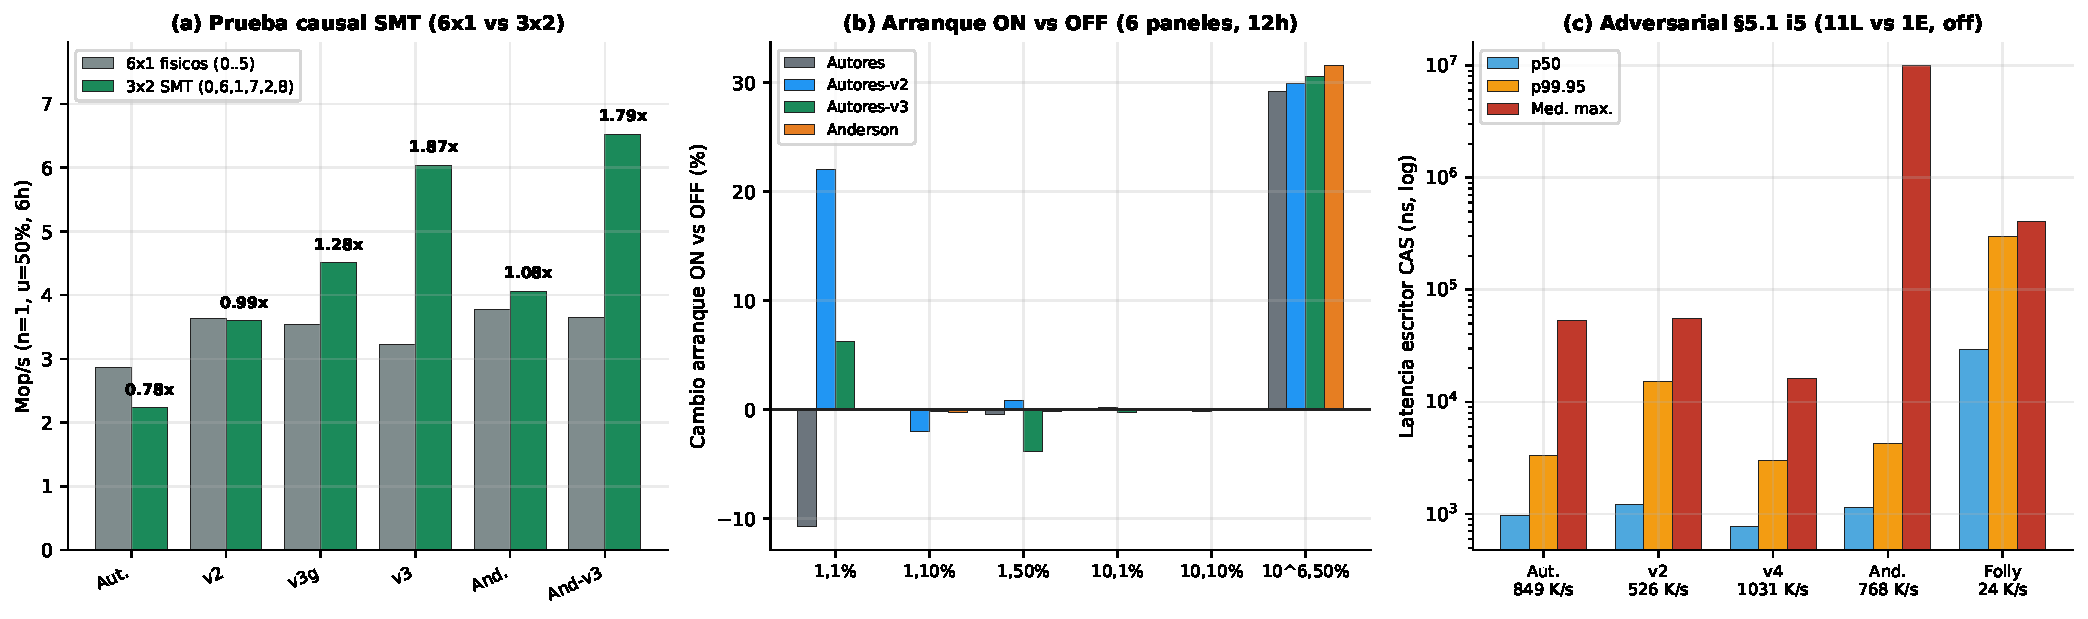
\includegraphics[width=\linewidth]{fig_i5_10400_mitigaciones_y_adversarial.pdf}
  \caption{(a) Prueba causal SMT en i5-10400 ($n=1, u=50\,\%$, 6 hilos, principal en \texttt{CPU 11}): \texttt{Autores-v3} gana $1{,}87\times$ al pasar de \texttt{6$\times$1} físicos a \texttt{3$\times$2} pares SMT mientras \texttt{Autores} cae $0{,}78\times$. (b) Cambio porcentual entre arranque \texttt{on} y \texttt{off} en los 6 paneles a 12\,h (incluyendo $n=1, u=1\,\%$). (c) Ataque adversarial \S 5.1 en i5-10400 (11 lectores vs.\ 1 escritor \texttt{CAS}, arranque \texttt{off}).}
  \label{fig:i5_miti_adv}
\end{figure}

% ==============================================================================
\section{Síntesis Final de las Cuatro Mejoras}
% ==============================================================================

\begin{table}[H]
\centering
\caption{Comparativa integrada de la evolución \texttt{Autores} $\to$ \texttt{v1} $\to$ \texttt{v2} $\to$ \texttt{v3} $\to$ \texttt{v4} en Intel Core Ultra 9 285.}
\label{tab:sintesis_final}
\resizebox{\linewidth}{!}{%
\begin{tabular}{@{}l c c c c c@{}}
\toprule
\textbf{Métrica clave (24 hilos)} & \textbf{Autores (orig.)} & \textbf{Autores-v1} & \textbf{Autores-v2} & \textbf{Autores-v3} & \textbf{Autores-v4} \\
\midrule
$n=1, u=50\,\%$ (Mop/s) & 0{,}96--1{,}03 & 1{,}48 & 1{,}63--1{,}72 & \textbf{3{,}66 ($3{,}81\times$)} & 1{,}49 \\
$n=10, u=10\,\%$ (Mop/s) & 51{,}39--55{,}51 & 53{,}51 & 55{,}54--56{,}28 & \textbf{73{,}83 ($1{,}44\times$)} & 47{,}98 \\
$n=10^6, u=50\,\%$ (Mop/s) & 47{,}31--48{,}21 & 49{,}30 & \textbf{65{,}98 ($1{,}39\times$)} & 64{,}09 & 63{,}71 \\
Pico RSS en $n=10^6$ (MB) & 1\,075 & 1\,075 & \textbf{760 ($-29{,}3\,\%$)} & 763 & 760 \\
Ataque E-core 23L+1E (\texttt{p99,95} / Kops/s) & 259\,$\mu$s / 98{,}7 & — & 549\,$\mu$s / 44{,}4 & — & \textbf{14{,}3\,$\mu$s / 210{,}0} \\
Memoria retenida (\texttt{bench\_basura}, 24\,h) & 54 (0 dif.) & 52 (0 dif.) & 53 (0 dif.) & 53 (0 dif.) & 55 (0 dif.) \\
\bottomrule
\end{tabular}%
}
\end{table}

Cada peldaño resuelve un cuello de botella distinto y medible de la réplica de Euro-Par 2024: \texttt{v1+v2} corrigen la implementación C++ oficial hasta dominar $n=10^6$ y la latencia P-core; \texttt{v3} convierte la topología híbrida L2+P/E de Arrow Lake en ventaja competitiva alcanzando liderazgo \textbf{6 de 6} frente a los algoritmos originales; y \texttt{v4} cierra la vulnerabilidad de inanición del \S 5.1 bajo ataques adversariales de lectores rápidos contra escritores en núcleos lentos.

\bibliographystyle{plain}
\bibliography{referencias_mejoras}

\end{document}
